\section{Theorie}
\label{sec:Theorie}

Die folgenden theoretischen Grundlagen stammen aus den Referenzen \cite{lasertheorie1}, \cite{lasertheorie2} und  \cite{lasertheorie3}

\subsection{Der Laser}
Laser steht für Light Amplification by Stimulated Emission of Radiation. Er wird verwendet wenn z.B. bei Interferenzeffekten kohärentes Licht erforderlich ist, das heißt, der Phasenunterschied der ausgesendeten Lichtwellen konstant sein muss.\\
Das Prinzip eines Lasers lässt sich an einem Zwei-Niveau-System beschreiben.
In einem Medium, für das ein angeregter Zustand $n_.1$ und ein Grundzustand $n_.0$ existieren, kann falls $n_.1$ besetzt ist unter spontaner Emission eines Photons das Material in den Grundzustand zurückkehren.
Trifft ein elektromagnetisches Feld darauf kann das Medium entweder durch Absorption des Photons in $n_.1$ übergehen, wenn dieses genau die Energie des Übergangs besitzt, oder der Prozess der Emission kann ohne Verlust des ankommenden Photons stimuliert werden. Das in diesem Fall freiwerdende Photon hat dann dieselbe Energie, Phase und Ausbreitungsrichtung wie das einfallende und ist somit kohärent zu diesem.
Die Zahl der absorbierten und emittierten Photonen pro Volumen und Zeit lässt sich mit den Einsteinkoeffizienten $A_.{21}$, $B_.{12}$ und $B_.{21}$, die die Übergangswahrscheinlichkeiten darstellen, und der elektromagnetischen Felddichte $\rho(\nu)$ schreiben als
\begin{align*}
\dot{N}_.E&=n_.1  A_.{21}\\
\dot{N}_.A&=n_.0 \rho(\nu) B_.{12}\\
\dot{N}_.{IE}&=n_.1 \rho(\nu) B_.{21},
\end{align*}
wobei der Index $A$ für die Absorption und die Indizes $E$ und $IE$ für die spontane bzw. induzierte Emission stehen.
Damit ergibt sich für die Änderung der Besetzung der Zustände
\[
\frac{\mathrm{d}n_.0}{\mathrm{d}t}=n_.1A_.{21}-n_.1 \rho(\nu) B_.{21}-n_.0 \rho(\nu) B_.{12}
\]
und 
\[
\frac{\mathrm{d}n_.1}{\mathrm{d}t}=-\frac{\mathrm{d}n_.0}{\mathrm{d}t}
\]
Nach der Maxwell-Boltzmann-Verteilung ist im thermischen Gleichgewicht vorwiegend der Grundzustand besetzt, sodass die stimulierte Emission eines Photons unwahrscheinlich ist.
Um eine konstante Verstärkung und Kohärenz zu erhalten, muss dem System deshalb ständig Energie zugeführt werden, damit die Besetzungsinversion $n_.1>n_.0$ auftritt. Dieser 'pumpen' genannte Vorgang wird über einen zusätzlichen Bestandteil des Lasers, das Pumpmaterial, gewährleistet, welches in diesem Versuch durch das Helium realisiert wird. Dies wird über über Anlegen einer Hochspannung angeregt und gibt die Energie über Stöße an das aktive Material ab.\\
Bisher wurde ein Zwei-Niveau-System betrachtet, welches jedoch nicht für einen Lasers geeignet ist. Sind die Zustände $n_.0$ und $n_.1$ nicht entartet, gilt $B_.{12}=B_.{21}$, sodass die Wahrscheinlichkeit für Absorption und stimulierte Emission gleich groß ist. Mit der Zeit stellt sich deshalb ein Gleichgewicht der Besetzungen ein und da zusätzlich durch spontane Emission mehr Elektronen aus dem höheren Zustand fallen, wird die Besetzungsinversion aufgehoben.\\ 
Ein Laser besteht neben dem aktiven Lasermaterial und einem Pumpmaterial aus einem optischen Resonator.
Dieser besteht aus einem totalreflektierenden Spiegel auf der einen und einem nur teilreflektierendem Spiegel auf der anderen Seite des Lasermediums und dient dazu, dass das emittierte Licht möglichst lange im aktiven Material verbleibt, um dort möglichst oft die induzierte Emission auszulösen. Der teilreflektierende Spiegel dient dazu den Laserstrahl auszukoppeln. Grundsätzlich können Resonatoren aus zwei planen oder zwei sphärischen Spiegeln oder einer Mischung aus beidem. Um Strahlungsverluste zu vermeiden, werden die Spiegel so aufgestellt, dass ihre Brennpunkte aufeinander liegen. Damit das System optisch stabil ist, also die Verluste geringer sind als die Verstärkung, muss für die Resonatorparameter
\[
g_.i = 1 - \frac{L}{r_.i}
\]
mit der Resonatorlänge $L$ und dem Krümmungsradius des jeweiligen Spiegels $r_.i$, gelten
\begin{equation}
0 \leq g_.1g_.2 < 1\text{.}\label{eq:stabil}
\end{equation}
Im Falle zweier gleichartig gekrümmter Spiegel beträgt die maximale Resonatorlänge $L_.{max}=r_.1+r_.2$.
Zum Herausfiltern einzelner zu verstärkender Wellenlängen können die Spiegel beschichtet werden, um die störenden Frequenzen zu absorbieren.

\subsection{TEM-Moden und longitudinale Moden}
Auf Grund von mehreren erreichbaren Energiezuständen können auch verschiedene Frequenzen die Resonanzbedingung \eqref{eq:stabil} erfüllen. Dadurch kann es zu mehreren Laser-Moden kommen, die in zylindrischer Symmetrie als transversale elektromagnetische (TEM) Moden bezeichnet werden.
Werden die Modenordnungen in radialer und Winkelrichtung  mit $p$ und $l$ bezeichnet ergibt sich die Intensität der TEM-Moden mit den Laguerre-Polynomen $L^q_.p$ zu
\begin{equation}
I_.{pl} \propto \cos^2 (l \varphi) \frac{(2\rho)^4}{(1+Z^2)^{(1+l)}} \left[L^q_.{p}\left(\frac{(2 \rho)^2}{1+Z^2} \right)\right] ^2 \exp\left(-\frac{2\rho^2}{1+Z^2} \right)\text{.} \label{eq:intens}
\end{equation}
Dabei ist
\[
\rho^2 = \frac{2\pi}{R\lambda}\text{ und } Z = \left(\frac{2z}{R}\right)
\]
Wird die Symmetrie durch ein Brewsterfenster gebrochen, um polarisiertes LASER-Licht zu erhalten werden werden die Ordnungen Moden in $x$- und $y$- Richtung mit $m$ und $n$ bezeichnet.
Die Intensität ergibt ich dann mit den Hermit-Polynomen $H_.m$ über
\begin{equation}
I_{mn} = I_.0 \left(\frac{w_0}{w}\right)^2 \left[H_.m\left(\frac{\sqrt{2} x}{w}\right) \exp\left(\frac{-x^2}{w^2}\right) \right]^2 \left[H_n\left(\frac{\sqrt{2} y}{w}\right) \exp\left(\frac{-y^2}{w^2}\right) \right]^2
\label{eq:intens2}
\end{equation}
mit dem Strahlradius $w$.
Dieser erfüllt die relation
\[
w (z) = w_0\sqrt{1+\left(\frac{z\lambda}{\pi}\right)^2}
\]
mit dem minimalen Strahlradius $w_0$.
Moden entlang der Symmetrieachse ($z$-Richtung) werden durch den Modenindex $q$ charakterisiert und als longitudinale elektromagnetische Moden (LEM) bezeichnet. Für reine longitudinale Moden $\text{LEM}_.{00q}$ gilt dabei
\begin{equation}
I_{00q} = I_0 \exp\left(-\frac{2 r^2}{\omega ^2}\right)\text{.} \label{eq:gaus}
\end{equation}

\subsection{Multimodenbetrieb}
Da die Resonatorlänge $L$ sehr viel größer als die Wellenlänge $\lambda$ des Lasers ist, erfüllen aufgrund der Dopplerverschiebung der Wellenlänge prinzipiell viele Frequenzen die Resonanzbedingung einer stehenden Welle im Resonator.
Denn die Wellenlänge des Lasers ist nicht monochromatisch, sondern Gaußverteilt um die Wellenlänge des induzierten Übergangs. \\
Die Geschwindigkeitsverteilung ist durch die Maxwell-Verteilung gegeben:
\[
P_v(v)=\sqrt{\frac{m_.N}{2\pi k_.BT}}\exp\left(-\frac{m_.Nv^2}{2k_.BT}\right)
\]
mit der Masse $m_.N$ von Neon, der Temperatur $T$ und der Boltzmann konstanten $k_.B$.
Die Doppler-Verschiebung ist gegeben durch 
\[
f = f_0\left(1+\frac{v}{c}\right)
\]
mit der Ruhefrequenz $f_0$ und der Lichtgeschwindigkeit $c$.
Auflösen nach $v$ ergibt die Frequenzabhängige Verteilung
\begin{align*}
P_f(f)&=\frac{c}{f_0}P_v\left(c\left(\frac{f}{f_0}-1\right)\right)\\
	&= \sqrt{\frac{m_.Nc^2}{2\pi k_.BT}}\exp\left(-\frac{m_.Nc^2(f-f_0)^2}{2k_.BTf_0^2}\right)
\end{align*}
Dies entspricht der genannten Gauß-Form.
Die Halbwertsbreite ist somit gegeben durch:
\[
\Delta f = \sqrt{\frac{8k_.BT\log(2)}{m_.Nc^2}}f_0
\]
Einsetzen von $f_0=c/\lambda_0$ mit $\lambda_0=\SI{632.8}{\nano\metre}$ bei Raumtemperatur $T=\SI{293.15}{\kelvin}$ ergibt:
\[
\Delta f = \SI{1.3}{\giga\hertz}\text{.}
\]
Vergleichsweise ist die Frequenzbreite der Resonator-Moden durch
\[
\Delta f_L = \frac{c}{2L} = \SI{375}{\mega\hertz}
\]
gegeben, also deutlich kleiner.
Folglich gibt es mehrere Wellenlängen die für eine gegebene Resonatorlänge $L$ die Bedingung 
\[
L = n\frac{\lambda}{2}
\]
erfüllen (vergleiche Abbildung \ref{fig:doppler}). Man spricht von einem Multimoden-Betrieb. 
Es gilt also für die Wellenlänge der stehenden Welle der Mode $q$
\[
\lambda_.q = \frac{2L}{q}\text{.}
\]
und für ihre Frequenz
\[
f_.q = q\frac{c}{2L}
\]
Das zeigt wie die Frequenz der entstehenden Moden abhängig von der Modenzahl $q$ ist. 
Der Frequenzabstand zwischen zwei benachbarten Moden $q$ und $q+1$ beträgt damit
\[
\Delta f = \frac{c}{2L}\text{.}
\]

\begin{figure}
	\centering
	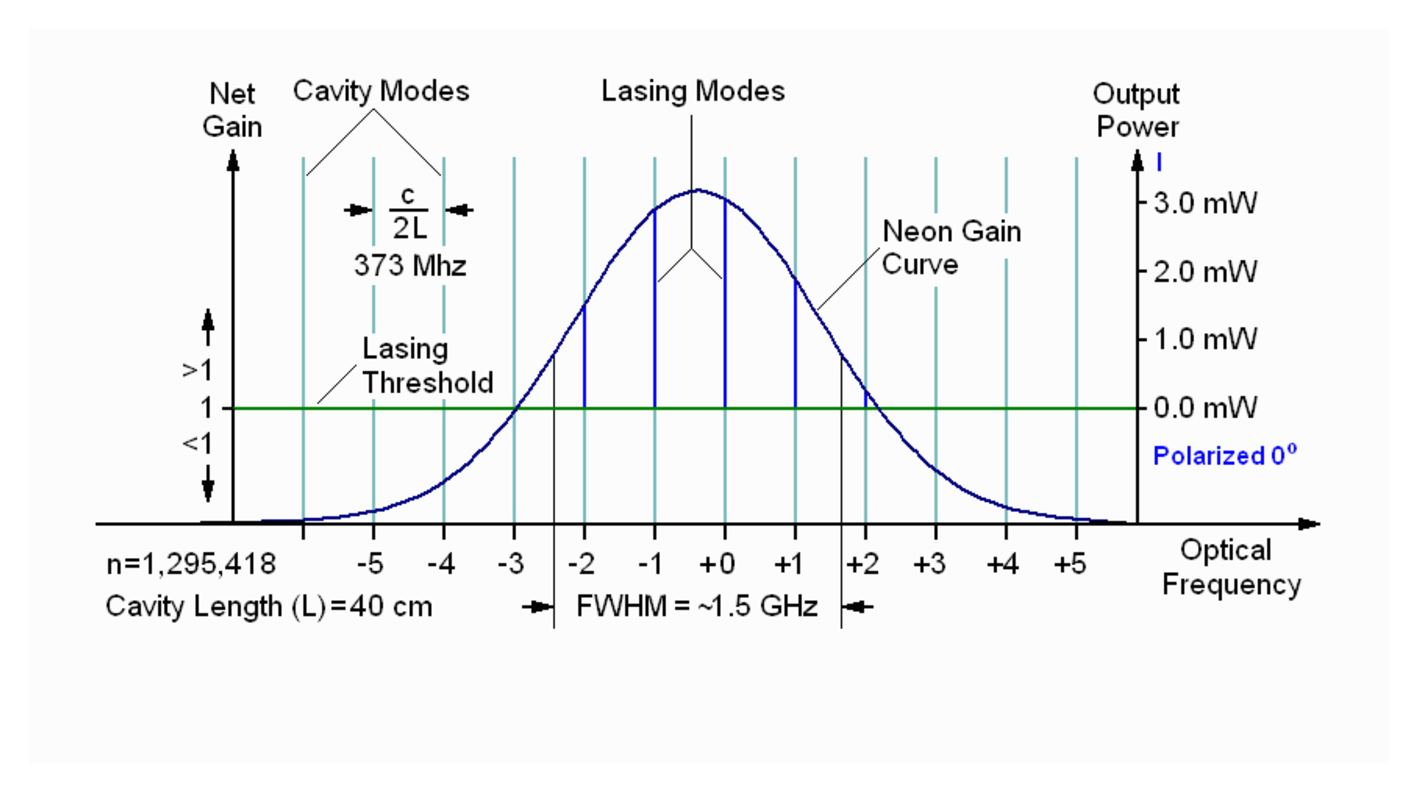
\includegraphics[width=\linewidth-50pt,height=\textheight-100pt,keepaspectratio]{content/images/multimode2.pdf}
	\caption{Longitudinale Moden eines typischen polarisierten $\SI{8}{\mega\watt}$ HeNe-Lasers.}
	\label{fig:doppler}
\end{figure}

\subsection{Intensität hinter einem Polarisationsfilter}
Ein Polarisationsfilter lässt nur eine Polarisationsrichtung passieren. Falls die Polarisation des Lichts sich um den Winkel $\delta\phi$ von dem gefilterten unterscheidet, gilt für die Intensität des Lichtes hinter diesem
\begin{equation}
	I=I_.0 cos^2(\delta\phi), \label{eq:polar}
\end{equation}
wobei $I_.0$ die Intensität vor dem Polarisationsfilter bezeichnet.


\subsection{Beugungsmuster verschiedener Wellenlängen am Gitter}
Durch das Einbringen des Gitters in den Lichtstrahl wird dieser am Gitter gebeugt. Dies führt zu Interferenzeffekten hinter dem Gitter. Es bilden sich Intensitätsmaxima aus. Aus den Abständen zwischen diesen und dem Abstand zum Schirm kann die Wellenlänge des Lichtstrahles folgendermaßen bestimmt werden
\begin{equation}
	\lambda = \frac{g \sin(\arctan(x/b))}{n}, \label{eq:lambda}
\end{equation}
wobei $g$ die Gitterkonstante, $x$ den Abstand des Hauptmaxima der Ordnung $n$ zur optischen Achse des ursprünglichen Strahles und $b$ der Abstand zwischen dem Schirm und dem Gitter ist.


